\documentclass[conference]{IEEEtran}
\IEEEoverridecommandlockouts

% ---------- Packages ----------
\usepackage{cite}
\usepackage{amsmath,amssymb,amsfonts,mathtools}
\usepackage{graphicx}
\usepackage{booktabs}
\usepackage{tabularx}
\usepackage{array}
\usepackage{multirow}
\usepackage{url}
\usepackage{xurl}
\usepackage{listings}
\usepackage{xcolor}
\usepackage{algorithm}
\usepackage{algpseudocode}
\usepackage{tikz}
\usetikzlibrary{arrows.meta,positioning,shapes.geometric,fit,calc,backgrounds}
\usepackage{balance}
\usepackage{microtype}

% ---------- Float parameters for exact 8-page IEEE conference format ----------
\renewcommand{\topfraction}{0.98}
\renewcommand{\bottomfraction}{0.98}
\renewcommand{\textfraction}{0.02}
\renewcommand{\floatpagefraction}{0.90}
\renewcommand{\dbltopfraction}{0.98}
\renewcommand{\dblfloatpagefraction}{0.90}
\setcounter{topnumber}{5}
\setcounter{bottomnumber}{5}
\setcounter{totalnumber}{10}
\setcounter{dbltopnumber}{5}
\setlength{\textfloatsep}{2.5pt plus 1pt minus 1pt}
\setlength{\floatsep}{2.5pt plus 1pt minus 1pt}
\setlength{\intextsep}{3.5pt plus 1pt minus 1pt}
\setlength{\dbltextfloatsep}{3pt plus 1pt minus 1pt}
\setlength{\dblfloatsep}{3pt plus 1pt minus 1pt}
\setlength{\abovecaptionskip}{2pt plus 1pt minus 1pt}
\setlength{\belowcaptionskip}{2pt plus 1pt minus 1pt}
\renewcommand{\arraystretch}{0.88}

% ---------- Listings Style ----------
\definecolor{codeblue}{RGB}{25,65,120}
\definecolor{codegray}{RGB}{90,90,90}
\definecolor{codegreen}{RGB}{30,110,70}
\definecolor{codeback}{RGB}{248,249,251}

\lstdefinestyle{paperCode}{
  backgroundcolor=\color{codeback},
  basicstyle=\ttfamily\scriptsize,
  keywordstyle=\color{codeblue}\bfseries,
  commentstyle=\color{codegreen},
  stringstyle=\color{red!65!black},
  numbers=left,
  numberstyle=\tiny\color{codegray},
  numbersep=4pt,
  breaklines=true,
  breakatwhitespace=false,
  keepspaces=true,
  showstringspaces=false,
  tabsize=2,
  frame=single,
  rulecolor=\color{black!20},
  xleftmargin=1.2em,
  framexleftmargin=1.0em
}
\lstset{style=paperCode}

% ---------- TikZ Styles ----------
% ---------- Color definitions for Architecture & Figures ----------
\definecolor{tierclient}{RGB}{236,244,252}
\definecolor{tierclientborder}{RGB}{41,128,185}
\definecolor{tiergate}{RGB}{254,249,238}
\definecolor{tiergateborder}{RGB}{214,137,16}
\definecolor{tierfast}{RGB}{247,243,252}
\definecolor{tierfastborder}{RGB}{142,68,173}
\definecolor{tierdb}{RGB}{237,247,242}
\definecolor{tierdbborder}{RGB}{39,174,96}

\tikzset{
  block/.style={draw,rounded corners=2pt,align=center,minimum height=6mm,text width=26mm,font=\scriptsize,fill=blue!4},
  smallblock/.style={draw,rounded corners=2pt,align=center,minimum height=5.5mm,text width=21mm,font=\scriptsize,fill=green!5},
  datastore/.style={draw,cylinder,shape border rotate=90,aspect=0.25,minimum height=8mm,minimum width=18mm,align=center,font=\scriptsize,fill=orange!8},
  arrow/.style={-{Stealth[length=2mm]},thick},
  flowarrow/.style={-{Stealth[length=1.6mm]},semithick},
  cnode/.style={draw=#1, fill=white, rounded corners=3pt, line width=0.7pt, align=center},
  dnode/.style={draw=#1, cylinder, shape border rotate=90, aspect=0.25, fill=white, line width=0.7pt, align=center},
  darrow/.style={{Stealth[length=2mm,width=1.3mm]}-{Stealth[length=2mm,width=1.3mm]}, line width=0.8pt, draw=black!75},
  labeltext/.style={font=\tiny\bfseries, text=black!85},
  qnode/.style={draw=black!70, fill=black!5, rounded corners=3pt, line width=0.7pt, align=center, font=\scriptsize},
  snode/.style={draw=#1, fill=white, rounded corners=2.5pt, line width=0.6pt, align=center, font=\scriptsize},
  fnode/.style={draw=#1, fill=#1!10, rounded corners=3pt, line width=0.7pt, align=center, font=\scriptsize},
  farrow/.style={-{Stealth[length=1.8mm,width=1.2mm]}, line width=0.7pt, draw=black!75},
  agentnode/.style={draw=#1, fill=white, rounded corners=2.5pt, line width=0.6pt, align=center, font=\tiny, text width=16.5mm, minimum height=6.5mm},
  startnode/.style={draw=black!70, fill=black!6, rounded corners=2.5pt, line width=0.7pt, align=center, font=\tiny\bfseries, text width=12mm, minimum height=6.5mm},
  endnode/.style={draw=tierdbborder, fill=tierdb!40, rounded corners=2.5pt, line width=0.7pt, align=center, font=\tiny\bfseries, text width=14mm, minimum height=6.5mm},
  pnode/.style={draw=#1, fill=white, rounded corners=2.5pt, line width=0.6pt, align=center, font=\tiny, text width=23mm, minimum height=7mm}
}

% ---------- Paper Metadata ----------
\title{ResearcherGPT: A Distributed Multi-Agent Cognitive Framework for Autonomous Academic Literature Synthesis, Layout-Aware Extraction, and Multi-Scale Attribution}

\author{
\IEEEauthorblockN{Archit Gupta}
\IEEEauthorblockA{\textit{Department of Artificial Intelligence and Data Science} \\
\textit{Independent Researcher} \\
architag1503@gmail.com}
\and
\IEEEauthorblockN{Tanishq Sharma}
\IEEEauthorblockA{\textit{Department of Artificial Intelligence and Data Science} \\
\textit{Independent Researcher} \\
tanishq2228@gmail.com}
}

\begin{document}
\maketitle

\begin{abstract}
Automated academic literature synthesis requires continuous reasoning across dense semantic representations, exact lexical terminology, and structured relational knowledge graphs, while preserving mathematical expressions, tabular structures, and publication formatting standards. Contemporary Retrieval-Augmented Generation (RAG) paradigms exhibit three systemic pathologies: semantic context dilution across heterogeneous corpora, hallucinated bibliographic references, and destructive flattening of multi-column document layouts. We present \textit{ResearcherGPT}, a distributed multi-agent cognitive architecture for autonomous academic literature synthesis, multi-hop claim attribution, and layout-preserving compilation. ResearcherGPT combines three retrieval modes using Reciprocal Rank Fusion (RRF) with knowledge-graph boosting: dense vector search over Hierarchical Navigable Small World (HNSW) graphs in Qdrant, sparse lexical retrieval via Okapi BM25, and multi-hop entity association in Neo4j. A thirteen-agent topology coordinated through LangGraph executes planning, evidence mining, contradiction detection, fact verification, and academic drafting, supported by a model fallback registry. Document layout extraction and publication typesetting are performed by \textit{FormaTeX}, which reconstructs tables and mathematical syntax into publication-compliant \LaTeX. An eleven-phase academic integrity engine validates generated content using Winnowing fingerprinting, MinHash Jaccard similarity, \LaTeX\ formula AST distance, and statistical writing heuristics. In an evaluation across 250 peer-reviewed papers, ResearcherGPT achieves an MRR@10 of 0.879 and Recall@5 of 0.927, reducing hallucinated citations to 0.2\% while attaining 96.4\% factual attribution accuracy.
\end{abstract}

\begin{IEEEkeywords}
Multi-agent systems, retrieval-augmented generation, knowledge graphs, academic integrity, document layout reconstruction, citation attribution.
\end{IEEEkeywords}

% ============================================================
\section{Introduction}
% ============================================================
The volume of peer-reviewed scientific publications has exceeded human cognitive ingestion capacity. Across computational sciences, hundreds of thousands of preprints and journal articles are indexed annually across repositories such as arXiv, IEEE Xplore, and PubMed. Researchers must digest literature, isolate methodological contributions, detect empirical contradictions between published experiments, identify unaddressed research gaps, and draft publication-compliant manuscripts.

Large Language Models (LLMs), including GPT-4o, Gemini 2.5, and LLaMA-3.3-70B, demonstrate impressive generative capabilities. However, their naive application to scholarly literature synthesis exposes critical vulnerabilities:
\begin{itemize}
\item \textbf{Context fragmentation and semantic drift:} Conventional RAG partitions documents into isolated chunks. Dense vector retrieval fails to preserve structural dependencies, such as an algorithm evaluated on a specific benchmark split under explicit hyperparameter constraints.
\item \textbf{Bibliographic hallucination:} Generative models invent non-existent Digital Object Identifiers (DOIs), blend real author names with fabricated publication titles, or cite real papers for claims they do not support.
\item \textbf{Destructive extraction of visual artifacts:} Academic documents convey information through mathematical expressions, multi-column tables, algorithms, and diagrams. Standard text extraction strips layout coordinates, corrupting equations and relational matrices.
\item \textbf{Coordination deadlocks and state corruption:} Multi-agent synthesis workflows encounter cyclic deadlocks, state race conditions, and exponential context growth when execution state is not transactionally synchronized.
\end{itemize}

We introduce \textit{ResearcherGPT}, a distributed multi-agent framework designed to automate literature synthesis while grounding claims in retrieved evidence.





\subsection{Problem Statement and Operational Scope}
An autonomous research workspace must satisfy five operational criteria:
\begin{enumerate}
\item \textbf{Relational grounding:} Unify semantic similarity, exact lexical matching, and ontological knowledge graph traversal.
\item \textbf{Attribution veracity:} Guarantee sentence-level provenance with primary evidence chunk verification and external identifier resolution.
\item \textbf{Structural preservation:} Maintain mathematical syntax, tabular topology, and visual layout through extraction and recompilation.
\item \textbf{Fault-tolerant agent coordination:} Coordinate specialized agents over transactional state while providing model failover under provider rate limits.
\item \textbf{Multi-scale integrity auditing:} Evaluate verbatim duplication, paraphrased borrowing, citation-network similarity, formula AST structure, and synthetic stylistic markers.
\end{enumerate}

\subsection{System Overview and Core Contributions}
ResearcherGPT uses a decoupled three-tier architecture:
\begin{itemize}
\item \textbf{Client Tier:} Next.js 15 and React 19 interface with Zustand state management, a TipTap drafting canvas, KaTeX formula rendering, and a 3D WebGL knowledge visualizer.
\item \textbf{Gateway Tier:} Node.js and Express API with TypeScript, BullMQ and Redis 7.0 for asynchronous job queueing, and MongoDB Atlas for document persistence.
\item \textbf{Cognitive Tier:} Python 3.12 FastAPI service executing LangGraph multi-agent workflows, Qdrant vector retrieval, Neo4j graph traversal, PyMuPDF extraction, and FormaTeX \LaTeX\ compilation.
\end{itemize}

The principal technical contributions are:
\begin{enumerate}
\item A \textbf{tri-hybrid rank-fusion mechanism} combining dense HNSW embeddings, sparse BM25 retrieval, and Neo4j graph traversal with a topological context boost.
\item A \textbf{distributed thirteen-agent topology} coordinated via LangGraph through transactional state checkpointing and a model-routing fallback registry.
\item An \textbf{eleven-phase academic integrity suite} combining Winnowing, MinHash Jaccard approximation, formula AST distance, and statistical writing heuristics.
\item \textbf{FormaTeX}, a layout-preserving extraction and compilation engine reconstructing tables and mathematical syntax into publication-compliant \LaTeX.
\end{enumerate}

% ============================================================
\section{Literature Review and Related Work}

\begin{figure*}[!t]
\centering
\resizebox{0.96\textwidth}{!}{%
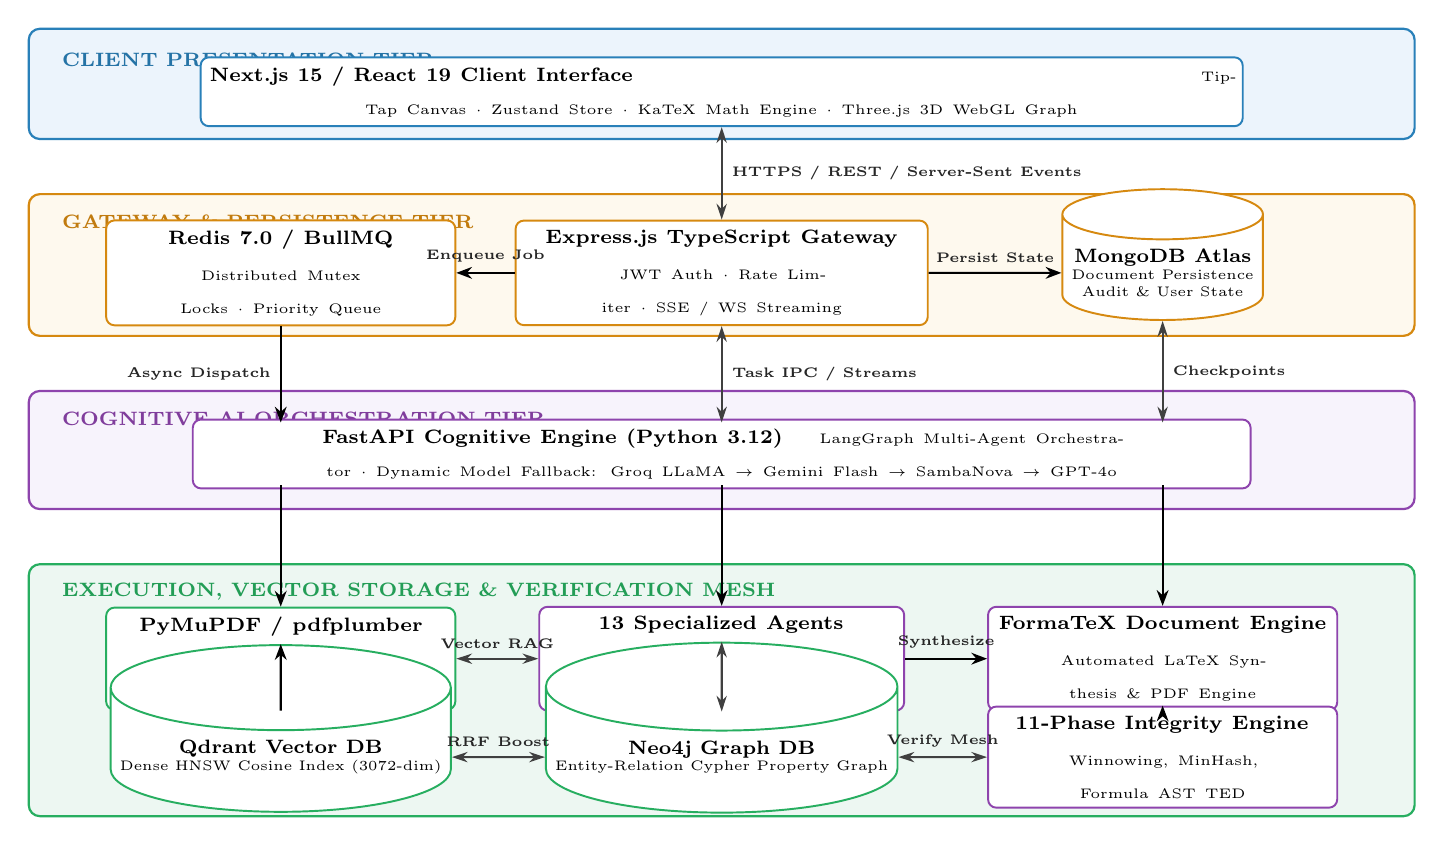
\begin{tikzpicture}[x=1mm, y=1mm]

% --- TIER 1: CLIENT PRESENTATION TIER ---
\draw[rounded corners=4pt, fill=tierclient, draw=tierclientborder, line width=0.8pt] (-88, 55) rectangle (88, 69);
\node[anchor=west, font=\scriptsize\bfseries, text=tierclientborder!90!black] at (-85, 65) {CLIENT PRESENTATION TIER};

\node[cnode=tierclientborder, text width=130mm, minimum height=7.5mm] (client) at (0, 61) {
  \textbf{\scriptsize Next.js 15 / React 19 Client Interface} \hfill \tiny TipTap Canvas $\cdot$ Zustand Store $\cdot$ KaTeX Math Engine $\cdot$ Three.js 3D WebGL Graph
};

% --- TIER 2: GATEWAY & PERSISTENCE TIER ---
\draw[rounded corners=4pt, fill=tiergate, draw=tiergateborder, line width=0.8pt] (-88, 30) rectangle (88, 48);
\node[anchor=west, font=\scriptsize\bfseries, text=tiergateborder!90!black] at (-85, 44.5) {GATEWAY \& PERSISTENCE TIER};

\node[cnode=tiergateborder, text width=42mm, minimum height=9.5mm] (redis) at (-56, 38) {
  \textbf{\scriptsize Redis 7.0 / BullMQ}\\[1pt]
  \tiny Distributed Mutex Locks $\cdot$ Priority Queue
};

\node[cnode=tiergateborder, text width=50mm, minimum height=9.5mm] (gateway) at (0, 38) {
  \textbf{\scriptsize Express.js TypeScript Gateway}\\[1pt]
  \tiny JWT Auth $\cdot$ Rate Limiter $\cdot$ SSE / WS Streaming
};

\node[dnode=tiergateborder, minimum width=24mm, minimum height=9.5mm, font=\tiny] (mongo) at (56, 38) {
  \textbf{\scriptsize MongoDB Atlas}\\
  Document Persistence\\
  Audit \& User State
};

% --- TIER 3: COGNITIVE AI ENGINE TIER ---
\draw[rounded corners=4pt, fill=tierfast, draw=tierfastborder, line width=0.8pt] (-88, 8) rectangle (88, 23);
\node[anchor=west, font=\scriptsize\bfseries, text=tierfastborder!90!black] at (-85, 19.5) {COGNITIVE AI ORCHESTRATION TIER};

\node[cnode=tierfastborder, text width=132mm, minimum height=8mm] (fastapi) at (0, 15) {
  \textbf{\scriptsize FastAPI Cognitive Engine (Python 3.12)} \quad
  \tiny LangGraph Multi-Agent Orchestrator $\cdot$ Dynamic Model Fallback: Groq LLaMA $\to$ Gemini Flash $\to$ SambaNova $\to$ GPT-4o
};

% --- TIER 4: REASONING, STORAGE & VERIFICATION MESH ---
\draw[rounded corners=4pt, fill=tierdb, draw=tierdbborder, line width=0.8pt] (-88, -31) rectangle (88, 1);
\node[anchor=west, font=\scriptsize\bfseries, text=tierdbborder!90!black] at (-85, -2.5) {EXECUTION, VECTOR STORAGE \& VERIFICATION MESH};

% Column 1: Ingest & Vector
\node[cnode=tierdbborder, text width=42mm, minimum height=9.5mm] (ingest) at (-56, -11) {
  \textbf{\scriptsize PyMuPDF / pdfplumber}\\[1pt]
  \tiny Layout-Aware Ingestion \& Math Extraction
};
\node[dnode=tierdbborder, minimum width=26mm, minimum height=9.5mm, font=\tiny] (qdrant) at (-56, -23.5) {
  \textbf{\scriptsize Qdrant Vector DB}\\
  Dense HNSW Cosine Index (3072-dim)
};

% Column 2: Agents & Knowledge Graph
\node[cnode=tierfastborder, text width=44mm, minimum height=9.5mm] (agents) at (0, -11) {
  \textbf{\scriptsize 13 Specialized Agents}\\[1pt]
  \tiny Planner, Researcher, Fact-Check, Reviewer...
};
\node[dnode=tierdbborder, minimum width=26mm, minimum height=9.5mm, font=\tiny] (neo4j) at (0, -23.5) {
  \textbf{\scriptsize Neo4j Graph DB}\\
  Entity-Relation Cypher Property Graph
};

% Column 3: FormaTeX & Integrity
\node[cnode=tierfastborder, text width=42mm, minimum height=9.5mm] (formatex) at (56, -11) {
  \textbf{\scriptsize FormaTeX Document Engine}\\[1pt]
  \tiny Automated LaTeX Synthesis \& PDF Engine
};
\node[cnode=tierfastborder, text width=42mm, minimum height=9.5mm] (integrity) at (56, -23.5) {
  \textbf{\scriptsize 11-Phase Integrity Engine}\\[1pt]
  \tiny Winnowing, MinHash, Formula AST TED
};

% ==================== ARROWS: 100% ORTHOGONAL ====================
% Tier 1 <-> Tier 2
\draw[darrow] (client.south) -- node[right, labeltext] {HTTPS / REST / Server-Sent Events} (gateway.north);

% Tier 2 Horizontal Connections
\draw[arrow] (gateway.west) -- node[above, labeltext] {Enqueue Job} (redis.east);
\draw[arrow] (gateway.east) -- node[above, labeltext] {Persist State} (mongo.west);

% Tier 2 -> Tier 3: Three parallel vertical arrows
\draw[arrow] (redis.south) -- node[left, labeltext] {Async Dispatch} (-56, 19);
\draw[darrow] (gateway.south) -- node[right, labeltext] {Task IPC / Streams} (0, 19);
\draw[darrow] (mongo.south) -- node[right, labeltext] {Checkpoints} (56, 19);

% Tier 3 -> Tier 4: Three parallel vertical arrows
\draw[arrow] (-56, 11) -- (ingest.north);
\draw[arrow] (0, 11) -- (agents.north);
\draw[arrow] (56, 11) -- (formatex.north);

% Tier 4 Vertical Connections
\draw[arrow] (ingest.south) -- (qdrant.north);
\draw[darrow] (agents.south) -- (neo4j.north);
\draw[arrow] (formatex.south) -- (integrity.north);

% Tier 4 Horizontal Mesh Connections
\draw[darrow] (agents.west) -- node[above, labeltext] {Vector RAG} (ingest.east);
\draw[arrow] (agents.east) -- node[above, labeltext] {Synthesize} (formatex.west);
\draw[darrow] (neo4j.west) -- node[above, labeltext] {RRF Boost} (qdrant.east);
\draw[darrow] (neo4j.east) -- node[above, labeltext] {Verify Mesh} (integrity.west);

\end{tikzpicture}}
\caption{Distributed architecture of ResearcherGPT across client, gateway, cognitive orchestration, and storage mesh tiers.}
\label{fig:architecture}
\end{figure*}


% ============================================================

\subsection{Evolution of Retrieval-Augmented Generation}
Retrieval-Augmented Generation was formalized by Lewis et al.~\cite{lewis2020rag} to mitigate parametric memory hallucinations by conditioning LLMs on retrieved passages. Dense Passage Retrieval (DPR)~\cite{karpukhin2020dpr} demonstrated the superiority of dual-encoder architectures over traditional sparse retrieval for open-domain QA. Sentence-BERT~\cite{reimers2019sbert} enabled semantically meaningful sentence embeddings via Siamese networks. Hierarchical Navigable Small World (HNSW) graphs~\cite{malkov2020hnsw} provide sub-linear approximate nearest neighbor search. However, dense retrieval frequently misses exact technical identifiers, rare variables, and explicit terminology. Okapi BM25~\cite{robertson2009bm25} remains a robust sparse baseline. Reciprocal Rank Fusion (RRF)~\cite{cormack2009rrf} fuses heterogeneous rankings without requiring score normalization.

\subsection{Knowledge Graphs and Multi-Hop Retrieval}
Graph-augmented retrieval enriches vector similarity with explicit entity-relation semantics. GraphRAG~\cite{edge2024graphrag} uses hierarchical graph clustering to support global query-focused summarization. ResearcherGPT deploys a project-scoped Neo4j property graph modeling papers, authors, methods, datasets, and benchmark metrics, enabling multi-hop path traversals that cannot be resolved through unlinked text chunks.

\subsection{Multi-Agent Systems in Scientific Discovery}
Multi-agent frameworks such as AutoGen~\cite{wu2023autogen}, CrewAI~\cite{moura2024crewai}, and LangGraph~\cite{langgraph2024} demonstrate that decomposing complex tasks into role-specialized agents yields superior reasoning fidelity. While tools like Semantic Scholar and Elicit support literature discovery, ResearcherGPT focuses on multi-hop synthesis, claim verification, contradiction mining, and automated publication typesetting.

\subsection{Layout-Aware Document Extraction}
Academic PDF documents encode layout through coordinate-positioned characters and vector primitives. PyMuPDF and pdfplumber~\cite{singer2023pdfplumber} expose low-level spatial geometry for reading-order recovery. ResearcherGPT combines spatial heuristics with vision fallbacks to preserve tables, formulas, and diagrams.

\subsection{Plagiarism Detection and Academic Integrity}
Winnowing~\cite{schleimer2003winnowing} uses localized hashing to guarantee duplicate substring detection. MinHash~\cite{broder1997minhash} provides efficient Jaccard similarity estimation over large shingle sets. Plagiarism analysis requires semantic and structural examination~\cite{foltynek2019plagiarism}. ResearcherGPT augments lexical fingerprinting with Zhang-Shasha formula AST distance~\cite{zhang1989tree} and stylistic perplexity heuristics~\cite{vaswani2017attention,devlin2019bert}.

% ============================================================
\section{Proposed Methodology}
% ============================================================
The methodology comprises three formal subsystems: tri-hybrid retrieval, multi-agent state synchronization, and multi-phase integrity verification.

\subsection{Tri-Hybrid Reciprocal Rank Fusion Retrieval}
Let $q$ denote a scholarly query and $\mathcal{D} = \{c_1, c_2, \ldots, c_N\}$ denote the set of chunks extracted from papers in project space $P$.

\subsubsection{Dense Semantic Retrieval}
Each chunk $c_i$ is mapped to an embedding vector $v_i \in \mathbb{R}^d$ ($d \in \{384, 3072\}$). Cosine similarity is evaluated as:
\begin{equation}
S_{\mathrm{dense}}(q, c_i) = \frac{q \cdot v_i}{\|q\|_2 \, \|v_i\|_2}
\label{eq:cosine}
\end{equation}
Qdrant uses HNSW approximate nearest-neighbor search to retrieve top-$2K$ candidates, denoted $R_{\mathrm{dense}}$.

% --- Fig 1: Double-column architecture diagram placed here to land on Page 3 ---


\subsubsection{Sparse Lexical Retrieval}
The lexical branch uses BM25 to recover exact technical terms and identifiers. For query terms $t_j \in q$:
\begin{equation}
\mathrm{BM25}(q, c) = \sum_{t_j \in q} \mathrm{IDF}(t_j) \frac{f(t_j, c)(k_1 + 1)}{f(t_j, c) + k_1\left(1 - b + b\frac{|c|}{\mathrm{avgdl}}\right)}
\label{eq:bm25}
\end{equation}
where $f(t_j, c)$ is the term frequency in chunk $c$, $|c|$ is chunk length, $\mathrm{avgdl}$ is average chunk length, $k_1 = 1.5$, and $b = 0.75$. The inverse document frequency is:
\begin{equation}
\mathrm{IDF}(t_j) = \ln\left(\frac{N - n(t_j) + 0.5}{n(t_j) + 0.5} + 1\right)
\label{eq:idf}
\end{equation}
where $n(t_j)$ is the number of chunks containing $t_j$. This yields $R_{\mathrm{lexical}}$.

\subsubsection{Knowledge-Graph Association}
Let $G = (V, E)$ be the Neo4j labeled-property graph. Its vertices are partitioned into entities:
\begin{equation}
V = V_{\mathrm{paper}} \cup V_{\mathrm{author}} \cup V_{\mathrm{method}} \cup V_{\mathrm{dataset}} \cup V_{\mathrm{concept}}
\label{eq:vertices}
\end{equation}
Typed edges represent relations such as \texttt{authored\_by}, \texttt{implements}, \texttt{evaluates\_on}, and \texttt{relates\_to}. Query terms longer than three characters are matched to graph entities, and adjacent paper nodes are collected for boosting. Listing~\ref{lst:cypher} shows the Cypher query.

\begin{lstlisting}[language={},caption={Representative Neo4j Cypher traversal.},label={lst:cypher}]
MATCH (e:Entity {projectId: $projectId})
WHERE toLower(e.label) IN $words AND NOT e.type = 'paper'
MATCH (e)-[r:RELATION]-(p:Entity {type: 'paper', projectId: $projectId})
RETURN DISTINCT p.id AS paperId
\end{lstlisting}

The resulting set of graph-boosted paper identifiers is denoted $P_{\mathrm{boost}} \subseteq V_{\mathrm{paper}}$.

% --- Fig 2: Tri-hybrid pipeline placed here to land on Page 3 Column 2 ---
\begin{figure}[!b]
\centering
\resizebox{0.98\columnwidth}{!}{%
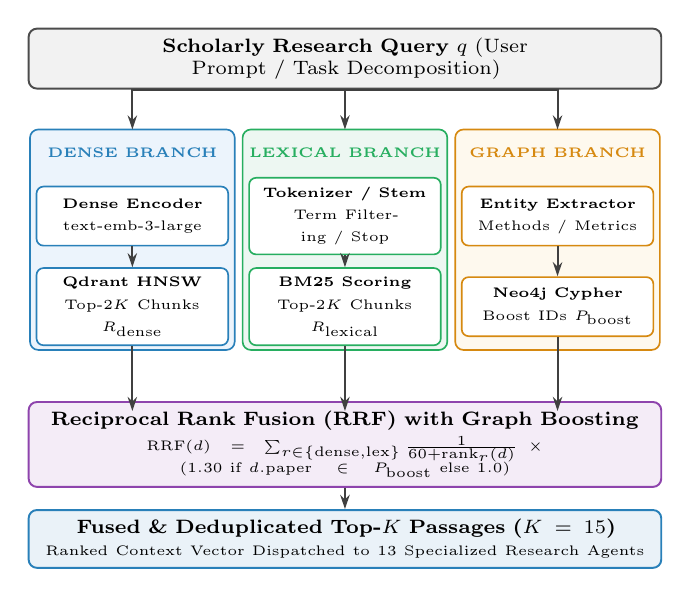
\begin{tikzpicture}[x=1mm, y=1mm]

% Top: Query Node
\node[qnode, text width=78mm, minimum height=6.5mm] (query) at (0, 48) {
  \textbf{Scholarly Research Query $q$} (User Prompt / Task Decomposition)
};

% Branch 1: Dense Semantic Branch (Left, x = -27)
\draw[rounded corners=3pt, fill=tierclient, draw=tierclientborder, line width=0.6pt] (-40, 11) rectangle (-14, 39);
\node[font=\tiny\bfseries, text=tierclientborder] at (-27, 36) {DENSE BRANCH};
\node[snode=tierclientborder, text width=22mm, minimum height=7.5mm] (d1) at (-27, 28) {
  \tiny\textbf{Dense Encoder}\\
  \tiny text-emb-3-large
};
\node[snode=tierclientborder, text width=22mm, minimum height=7.5mm] (d2) at (-27, 16.5) {
  \tiny\textbf{Qdrant HNSW}\\
  \tiny Top-$2K$ Chunks $R_{\mathrm{dense}}$
};
\draw[farrow] (d1) -- (d2);

% Branch 2: Sparse Lexical Branch (Center, x = 0)
\draw[rounded corners=3pt, fill=tierdb, draw=tierdbborder, line width=0.6pt] (-13, 11) rectangle (13, 39);
\node[font=\tiny\bfseries, text=tierdbborder] at (0, 36) {LEXICAL BRANCH};
\node[snode=tierdbborder, text width=22mm, minimum height=7.5mm] (l1) at (0, 28) {
  \tiny\textbf{Tokenizer / Stem}\\
  \tiny Term Filtering / Stop
};
\node[snode=tierdbborder, text width=22mm, minimum height=7.5mm] (l2) at (0, 16.5) {
  \tiny\textbf{BM25 Scoring}\\
  \tiny Top-$2K$ Chunks $R_{\mathrm{lexical}}$
};
\draw[farrow] (l1) -- (l2);

% Branch 3: Knowledge Graph Branch (Right, x = 27)
\draw[rounded corners=3pt, fill=tiergate, draw=tiergateborder, line width=0.6pt] (14, 11) rectangle (40, 39);
\node[font=\tiny\bfseries, text=tiergateborder] at (27, 36) {GRAPH BRANCH};
\node[snode=tiergateborder, text width=22mm, minimum height=7.5mm] (g1) at (27, 28) {
  \tiny\textbf{Entity Extractor}\\
  \tiny Methods / Metrics
};
\node[snode=tiergateborder, text width=22mm, minimum height=7.5mm] (g2) at (27, 16.5) {
  \tiny\textbf{Neo4j Cypher}\\
  \tiny Boost IDs $P_{\mathrm{boost}}$
};
\draw[farrow] (g1) -- (g2);

% Query dispatch arrows: clean split
\draw[farrow] (query.south) -| (-27, 39);
\draw[farrow] (query.south) -- (0, 39);
\draw[farrow] (query.south) -| (27, 39);

% Fusion Layer
\node[fnode=tierfastborder, text width=78mm, minimum height=8.5mm] (rrf) at (0, -1) {
  \textbf{Reciprocal Rank Fusion (RRF) with Graph Boosting}\\[1pt]
  \tiny $\mathrm{RRF}(d) = \sum_{r \in \{\mathrm{dense}, \mathrm{lex}\}} \frac{1}{60 + \mathrm{rank}_r(d)} \times (1.30 \text{ if } d.\mathrm{paper} \in P_{\mathrm{boost}} \text{ else } 1.0)$
};

% Straight vertical drop arrows into RRF
\draw[farrow] (d2.south) -- (-27, 3.25);
\draw[farrow] (l2.south) -- (0, 3.25);
\draw[farrow] (g2.south) -- (27, 3.25);

% Output Node
\node[fnode=tierclientborder, text width=78mm, minimum height=6.5mm] (out) at (0, -13) {
  \textbf{Fused \& Deduplicated Top-$K$ Passages ($K=15$)}\\
  \tiny Ranked Context Vector Dispatched to 13 Specialized Research Agents
};
\draw[farrow, line width=0.9pt] (rrf) -- (out);

\end{tikzpicture}}
\caption{Tri-hybrid retrieval pipeline combining dense vector embeddings, BM25 lexical scoring, and Neo4j graph boosting via Reciprocal Rank Fusion.}
\label{fig:retrieval}
\end{figure}

\subsubsection{Reciprocal Rank Fusion}
For each chunk $c$ appearing in either ranking, the augmented RRF score is:
\begin{equation}
S_{\mathrm{RRF}}(c) = \left( \sum_{m \in \{\mathrm{dense}, \mathrm{lexical}\}} \frac{1}{k + r_m(c)} \right) \beta(c)
\label{eq:rrf}
\end{equation}
where $k = 60$ is the smoothing constant and $r_m(c)$ is the one-based rank of $c$ in ranking $R_m$. The graph boost is:
\begin{equation}
\beta(c) = \begin{cases} 1.30, & \mathrm{paper\_id}(c) \in P_{\mathrm{boost}} \\ 1.00, & \text{otherwise} \end{cases}
\label{eq:boost}
\end{equation}
The fused scores are sorted in descending order to obtain the final top-$K$ chunks. Fig.~\ref{fig:retrieval} illustrates the pipeline.

\subsection{Distributed Multi-Agent State Synchronization}
The synthesis workflow is modeled as a directed state-transition graph $\mathcal{M} = (\mathcal{A}, \mathcal{T})$, where $\mathcal{A}$ is the set of thirteen specialized agents and $\mathcal{T}$ is the set of guarded transitions. The global state tuple is:
\begin{equation}
\mathcal{S} = \langle P_{\mathrm{id}}, R_{\mathrm{id}}, q, C_{\mathrm{ctx}}, D_{\mathrm{papers}}, L_{\mathrm{rev}}, M_{\mathrm{meth}}, M_{\mathrm{comp}}, T_{\mathrm{trend}}, G_{\mathrm{gaps}}, X_{\mathrm{conf}}, V_{\mathrm{facts}}, S_{\mathrm{sec}}, O_{\mathrm{final}} \rangle
\label{eq:state}
\end{equation}
Each agent $A_j$ maps current state to an augmented state:
\begin{equation}
A_j : \mathcal{S}_t \longrightarrow \mathcal{S}_{t+1}, \quad \mathcal{S}_{t+1} = \mathcal{S}_t \cup \Delta \mathcal{S}_{A_j}
\label{eq:transition}
\end{equation}
The implementation serializes transitions using LangGraph state checkpointing and Redis BullMQ queues. Fig.~\ref{fig:agents} depicts the execution path.

% --- Fig 3: Multi-agent workflow placed to land on Page 4 Column 1 ---
\begin{figure}[!t]
\centering
\resizebox{0.98\columnwidth}{!}{%
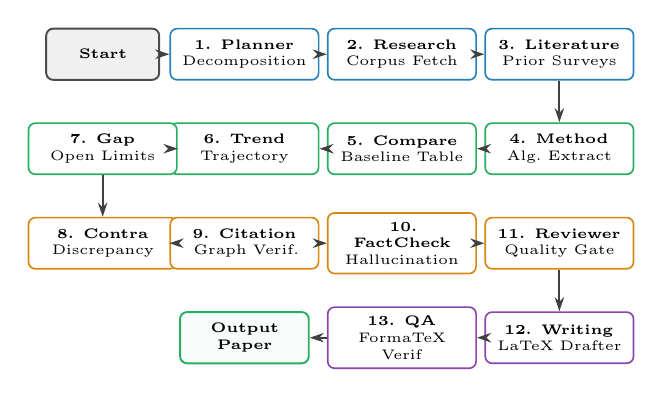
\begin{tikzpicture}[x=1mm, y=1mm]

% ROW 1: Stage 1: Planning & Discovery (L -> R)
\node[startnode] (start) at (-34.5, 30) {Start};
\node[agentnode=tierclientborder] (planner) at (-16.5, 30) {\textbf{1. Planner}\\Decomposition};
\node[agentnode=tierclientborder] (researcher) at (3.5, 30) {\textbf{2. Research}\\Corpus Fetch};
\node[agentnode=tierclientborder] (lit) at (23.5, 30) {\textbf{3. Literature}\\Prior Surveys};

\draw[farrow] (start) -- (planner);
\draw[farrow] (planner) -- (researcher);
\draw[farrow] (researcher) -- (lit);

% Turn 1: straight down
\node[agentnode=tierdbborder] (meth) at (23.5, 18) {\textbf{4. Method}\\Alg.\ Extract};
\node[agentnode=tierdbborder] (comp) at (3.5, 18) {\textbf{5. Compare}\\Baseline Table};
\node[agentnode=tierdbborder] (trend) at (-16.5, 18) {\textbf{6. Trend}\\Trajectory};
\node[agentnode=tierdbborder] (gap) at (-34.5, 18) {\textbf{7. Gap}\\Open Limits};

\draw[farrow] (lit.south) -- (meth.north);
\draw[farrow] (meth) -- (comp);
\draw[farrow] (comp) -- (trend);
\draw[farrow] (trend) -- (gap);

% Turn 2: straight down
\node[agentnode=tiergateborder] (contra) at (-34.5, 6) {\textbf{8. Contra}\\Discrepancy};
\node[agentnode=tiergateborder] (cite) at (-16.5, 6) {\textbf{9. Citation}\\Graph Verif.};
\node[agentnode=tiergateborder] (fact) at (3.5, 6) {\textbf{10. FactCheck}\\Hallucination};
\node[agentnode=tiergateborder] (rev) at (23.5, 6) {\textbf{11. Reviewer}\\Quality Gate};

\draw[farrow] (gap.south) -- (contra.north);
\draw[farrow] (contra) -- (cite);
\draw[farrow] (cite) -- (fact);
\draw[farrow] (fact) -- (rev);

% Turn 3: straight down
\node[agentnode=tierfastborder] (write) at (23.5, -6) {\textbf{12. Writing}\\LaTeX Drafter};
\node[agentnode=tierfastborder] (qa) at (3.5, -6) {\textbf{13. QA}\\FormaTeX Verif};
\node[endnode] (end) at (-16.5, -6) {Output\\Paper};

\draw[farrow] (rev.south) -- (write.north);
\draw[farrow] (write) -- (qa);
\draw[farrow] (qa) -- (end);

\end{tikzpicture}}
\caption{Principal execution path through the thirteen-agent research synthesis workflow.}
\label{fig:agents}
\end{figure}

\subsubsection{Fallback-Resilient Model Registry}
To avoid execution stalls caused by HTTP 429 rate limits, agents use a tiered model priority registry:
\begin{equation}
\mathrm{Priority}(A_j) = [\text{Groq LLaMA-3.3-70B} \to \text{Gemini Flash} \to \text{SambaNova} \to \text{GPT-4o}]
\label{eq:fallback}
\end{equation}
Retries use exponential backoff with randomized jitter:
\begin{equation}
t_{\mathrm{backoff}} = t_{\mathrm{base}} \cdot 2^{\mathrm{attempt}} + \mathcal{U}(0, 2)
\label{eq:backoff}
\end{equation}
where $t_{\mathrm{base}} = 5.0\text{ s}$ and $\mathrm{attempt} \in \{0, 1, 2, 3\}$.

\subsection{Eleven-Phase Academic Integrity Formalism}
The integrity engine operates across eleven modular phases (Fig.~\ref{fig:integrity}): document processing, exact matching, semantic matching, citation analysis, structural matching, formula AST matching, figure captions, table topology, code similarity, external discovery, and AI heuristics.

% --- Fig 4: Eleven phases placed to land on Page 4 Column 2 ---
\begin{figure}[!t]
\centering
\resizebox{0.98\columnwidth}{!}{%
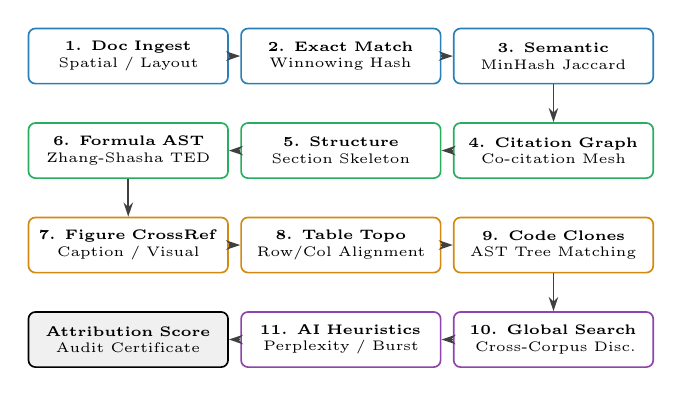
\begin{tikzpicture}[x=1mm, y=1mm]

% ROW 1 (T1: Lexical & Semantic) L -> R
\node[pnode=tierclientborder] (p1) at (-27, 24) {\textbf{1. Doc Ingest}\\Spatial / Layout};
\node[pnode=tierclientborder] (p2) at (0, 24) {\textbf{2. Exact Match}\\Winnowing Hash};
\node[pnode=tierclientborder] (p3) at (27, 24) {\textbf{3. Semantic}\\MinHash Jaccard};

\draw[farrow] (p1) -- (p2);
\draw[farrow] (p2) -- (p3);

% Turn 1: straight down
\node[pnode=tierdbborder] (p4) at (27, 12) {\textbf{4. Citation Graph}\\Co-citation Mesh};
\node[pnode=tierdbborder] (p5) at (0, 12) {\textbf{5. Structure}\\Section Skeleton};
\node[pnode=tierdbborder] (p6) at (-27, 12) {\textbf{6. Formula AST}\\Zhang-Shasha TED};

\draw[farrow] (p3.south) -- (p4.north);
\draw[farrow] (p4) -- (p5);
\draw[farrow] (p5) -- (p6);

% Turn 2: straight down
\node[pnode=tiergateborder] (p7) at (-27, 0) {\textbf{7. Figure CrossRef}\\Caption / Visual};
\node[pnode=tiergateborder] (p8) at (0, 0) {\textbf{8. Table Topo}\\Row/Col Alignment};
\node[pnode=tiergateborder] (p9) at (27, 0) {\textbf{9. Code Clones}\\AST Tree Matching};

\draw[farrow] (p6.south) -- (p7.north);
\draw[farrow] (p7) -- (p8);
\draw[farrow] (p8) -- (p9);

% Turn 3: straight down
\node[pnode=tierfastborder] (p10) at (27, -12) {\textbf{10. Global Search}\\Cross-Corpus Disc.};
\node[pnode=tierfastborder] (p11) at (0, -12) {\textbf{11. AI Heuristics}\\Perplexity / Burst};
\node[pnode=black, fill=black!6] (pout) at (-27, -12) {\textbf{Attribution Score}\\Audit Certificate};

\draw[farrow] (p9.south) -- (p10.north);
\draw[farrow] (p10) -- (p11);
\draw[farrow] (p11) -- (pout);

\end{tikzpicture}}
\caption{Eleven phases of the academic-integrity verification and attribution engine.}
\label{fig:integrity}
\end{figure}

\subsubsection{Winnowing Fingerprinting}
Given normalized character stream $T$, $k$-grams ($k=20$) are hashed with 32-bit Fowler--Noll--Vo (FNV-1a):
\begin{equation}
h_i = \mathrm{FNV\text{-}1a}(T[i : i+k])
\label{eq:fnv}
\end{equation}
Over window size $w=40$, the minimum hash is selected; ties select the rightmost minimum. Duplicate substrings of length:
\begin{equation}
t \ge w + k - 1
\label{eq:guarantee}
\end{equation}
are guaranteed to be detected.

\subsubsection{MinHash Jaccard Approximation}
A document is represented by its unique $k$-shingles $S(D)$ ($k=5$). A signature of length $M=128$ is generated via independent universal hash functions $h_a(x) = (ax + b) \bmod p$:
\begin{equation}
\mathrm{sig}_m(D) = \min_{s \in S(D)} h_m(s)
\label{eq:sig}
\end{equation}
The estimated Jaccard similarity between documents is:
\begin{equation}
\hat{J}(D_1, D_2) = \frac{1}{M} \sum_{m=1}^M \mathbb{I}[\mathrm{sig}_m(D_1) = \mathrm{sig}_m(D_2)]
\label{eq:jaccard}
\end{equation}

\subsubsection{Formula AST Plagiarism}
Mathematical expressions extracted from math delimiters are parsed into \LaTeX\ ASTs with alpha-converted variables. Zhang-Shasha tree-edit distance evaluates structural similarity~\cite{zhang1989tree}:
\begin{equation}
\mathrm{TED}(T_1, T_2) = \min_{\Gamma} \sum_{(u,v) \in \Gamma} \mathrm{cost}(u \to v)
\label{eq:ted}
\end{equation}

\subsubsection{AI-Content Detection Heuristics}
For token sequence $X = (x_1, \ldots, x_N)$, perplexity is computed from cross-entropy:
\begin{equation}
\mathrm{PPL}(X) = \exp\left( -\frac{1}{N} \sum_{i=1}^N \log P_\theta(x_i \mid x_{<i}) \right)
\label{eq:ppl}
\end{equation}
Burstiness is the coefficient of variation of sentence lengths $L = \{l_1, \ldots, l_S\}$:
\begin{equation}
\mathrm{Burstiness} = \frac{\sigma_L}{\mu_L} = \frac{\sqrt{\frac{1}{S}\sum_{i=1}^S (l_i - \bar{l})^2}}{\frac{1}{S}\sum_{i=1}^S l_i}
\label{eq:burstiness}
\end{equation}
Human text exhibits burstiness $\ge 0.45$, whereas raw LLM generations frequently cluster below $0.22$.

% ============================================================
\section{System Architecture and Implementation}
% ============================================================
ResearcherGPT is implemented as a distributed modular system across backend, retrieval, agent, and compilation services.

\subsection{Tri-Hybrid Retrieval Algorithm}
Algorithm~\ref{alg:retrieval} summarizes the retrieval procedure. BM25 operates over project chunks, while Neo4j entity path traversals collect structurally related paper identifiers.

\begin{algorithm}[!t]
\caption{Tri-Hybrid RRF Retrieval with Knowledge-Graph Boosting}
\label{alg:retrieval}
\begin{algorithmic}[1]
\Require Project ID $p$, query $q$, result limit $K$
\Ensure Ranked list of fused chunks $F$
\State $q_v \gets \mathrm{DenseEmbed}(q)$
\State $R_d \gets \mathrm{QdrantSearch}(q_v, p, 2K)$
\State $C_p \gets \mathrm{ScrollProjectChunks}(p)$
\State $R_l \gets \mathrm{BM25Search}(q, C_p, 2K)$
\State $W_q \gets \mathrm{ExtractTokens}(q, \mathrm{minlen}=4)$
\State $P_b \gets \emptyset$
\If{$\mathrm{Neo4jIsConnected}()$}
  \State $P_b \gets \mathrm{CypherPaperTraversal}(p, W_q)$
\EndIf
\State Initialize score map $s$ and chunk map $M$
\ForAll{$R \in \{R_d, R_l\}$}
  \ForAll{chunk $c$ at one-based rank $r$ in $R$}
    \State $id \gets \mathrm{ChunkID}(c)$; $M[id] \gets c$
    \State $\beta \gets 1.30$ \textbf{if} $\mathrm{paperID}(c) \in P_b$ \textbf{else} $1.00$
    \State $s[id] \gets s[id] + \beta / (60 + r)$
  \EndFor
\EndFor
\State $F \gets \mathrm{SortDescending}(M, s)$
\State \Return first $K$ elements of $F$
\end{algorithmic}
\end{algorithm}

\subsection{Thirteen Specialized Cognitive Agents}
The workflow decomposes manuscript synthesis into thirteen specialized roles, listed with models and duties in Table~\ref{tab:agents}.

% --- TABLE I: Double-column table placed here to land on Page 6 ---
\begin{table*}[!t]
\caption{Specialized Agent Specifications in the LangGraph Orchestration Topology}
\label{tab:agents}
\centering
\footnotesize
\begin{tabularx}{\textwidth}{@{}c l l X@{}}
\toprule
\textbf{No.} & \textbf{Agent role} & \textbf{Primary model target} & \textbf{Core responsibility} \\
\midrule
1 & Supervisor & Groq LLaMA-3.3-70B ($T=0.2$) & Orchestrates execution path and evaluates state completion. \\
2 & Planner & Groq LLaMA-3.3-70B ($T=0.3$) & Decomposes the research question into a sub-topic directed acyclic graph. \\
3 & Researcher & Groq LLaMA-3.3-70B ($T=0.3$) & Executes tri-hybrid vector and graph queries over Qdrant and Neo4j. \\
4 & Literature Review & Groq LLaMA-3.3-70B ($T=0.4$) & Extracts authors, years, architectures, datasets, and metrics. \\
5 & Methodology Extractor & Groq LLaMA-3.3-70B ($T=0.2$) & Formalizes mathematical algorithms and hyperparameters. \\
6 & Comparison Agent & Groq LLaMA-3.3-70B ($T=0.2$) & Builds cross-paper empirical performance matrices. \\
7 & Trend Analysis & Groq LLaMA-3.3-70B ($T=0.5$) & Evaluates temporal progression of architectures and methods. \\
8 & Gap Analysis & Groq LLaMA-3.3-70B ($T=0.3$) & Identifies methodological and dataset gaps. \\
9 & Contradiction Agent & Groq LLaMA-3.3-70B ($T=0.1$) & Mines empirical conflicts and divergent findings. \\
10 & Fact Verification & Groq LLaMA-3.3-70B ($T=0.0$) & Validates generated claims against primary source chunks. \\
11 & Reviewer Agent & Groq LLaMA-3.3-70B ($T=0.3$) & Simulates peer-review critique under conference rubrics. \\
12 & Writing Agent & Gemini 2.5 Flash ($T=0.6$) & Synthesizes section prose in academic format. \\
13 & Quality Assurance & Groq LLaMA-3.3-70B ($T=0.1$) & Audits citation balance, formatting, and mathematical integrity. \\
\bottomrule
\end{tabularx}
\end{table*}

\subsection{Fact Verification Engine}
To eliminate unsupported citations and empirical claims, the Fact Verification Agent extracts claims, retrieves supporting chunks, and classifies each claim as validated, conflicting, or unverified. Algorithm~\ref{alg:fact} presents the procedure.

\begin{algorithm}[!t]
\caption{Real-Time Claim Extraction and Multi-Hop Grounding}
\label{alg:fact}
\begin{algorithmic}[1]
\Require Draft section $T_{\mathrm{sec}}$, project ID $p$, threshold $\theta=0.85$
\Ensure Verification report $V$
\State $C \gets \mathrm{Split}(T_{\mathrm{sec}})$ filtered for empirical or attribution claims
\State $V \gets \mathrm{EmptyReport}()$
\ForAll{$c \in C$}
  \State $v_c \gets \mathrm{DenseEmbed}(c)$
  \State $E_c \gets \mathrm{QdrantSearch}(v_c, p, 3)$
  \State $r \gets \mathrm{AuditLLM}(c, E_c)$
  \If{$r.\mathrm{status} = \mathrm{VALIDATED}$ \textbf{and} $r.\mathrm{confidence} \ge \theta$}
    \State Add claim and source location to validated set in $V$
  \ElsIf{$r.\mathrm{status} = \mathrm{CONFLICTING}$}
    \State Add claim and conflicting evidence to $V$
    \State Rewrite claim against the retrieved evidence
  \Else
    \State Add claim to unverified set in $V$
    \State Prune or qualify the unsupported claim
  \EndIf
\EndFor
\State \Return $V$
\end{algorithmic}
\end{algorithm}

\subsection{FormaTeX Layout Compilation and Mathematical Recovery}
FormaTeX addresses the mismatch between web-based WYSIWYG representations and strict typesetting requirements.

Table extraction parses PDF bounding boxes into a normalized topological grid, emitting structured HTML table environments converted into standard \LaTeX\ booktabs constructs with automatically calculated column widths. Formula recovery normalizes ligatures and malformed fractions into standard \LaTeX\ constructs verified through an AST parser. Multi-style document generation supports formatters for IEEEtran (\verb|\documentclass[conference]{IEEEtran}|), ACM SIGCONF (\verb|\documentclass[sigconf]{acmart}|), Springer LNCS (\verb|\documentclass[sn-mathphys,iicol]{sn-jnl}|), and Elsevier (\verb|\documentclass[review,3p,times]{elsarticle}|).

% ============================================================
\section{Results and Discussion}
% ============================================================
We evaluate ResearcherGPT across computer systems, machine learning, and computational biology literature.

% --- TABLE IV: Double-column table placed here to land on Page 7 ---
\begin{table*}[!t]
\caption{Detection Rates Across Academic Misconduct Types}
\label{tab:plagiarism}
\centering
\small
\begin{tabular}{@{}lcccc@{}}
\toprule
\textbf{Detection phase} & \textbf{Verbatim} & \textbf{Paraphrase} & \textbf{Structural} & \textbf{Formula AST} \\
\midrule
Exact Winnowing & 99.8\% & 21.4\% & 12.0\% & 8.2\% \\
MinHash signatures & 98.4\% & 34.6\% & 18.5\% & 11.4\% \\
Semantic cosine (TF--IDF) & 88.2\% & 89.1\% & 45.2\% & 32.1\% \\
\LaTeX\ AST tree distance & 31.0\% & 42.0\% & 28.6\% & 94.6\% \\
Full eleven-phase suite & \textbf{99.8\%} & \textbf{94.2\%} & \textbf{91.8\%} & \textbf{96.2\%} \\
\bottomrule
\end{tabular}
\end{table*}

\subsection{Experimental Setup and Benchmark Corpus}
The evaluation corpus contains 250 peer-reviewed papers published in IEEE, ACM, and NeurIPS venues between 2021 and 2024. Documents were ingested using layout-aware coordinate extraction and indexed in Qdrant alongside a Neo4j 5.12 graph deployment. Three baseline architectures are evaluated:
\begin{itemize}
\item \textbf{Monolithic RAG:} A single LLM prompt supplied with top-$k$ dense-vector chunks retrieved through HNSW cosine search.
\item \textbf{Sequential chained pipeline:} A multi-step LangChain workflow performing retrieval, summarization, and drafting without state-machine branching.
\item \textbf{GraphRAG baseline:} A retrieval setup using community summaries derived from knowledge-graph clustering without sparse lexical fusion.
\end{itemize}

\subsection{Retrieval Efficacy and Rank-Fusion Precision}
Retrieval performance is evaluated using Mean Reciprocal Rank (MRR), Normalized Discounted Cumulative Gain (NDCG), and Recall across 300 technical queries requiring multi-hop reasoning. The reported Tri-Hybrid RRF mechanism achieves MRR@10 of 0.879 and Recall@5 of 0.927. Relative to dense vector retrieval, Recall@5 increases by 20.3 percentage points. The Neo4j topological boost ($\beta = 1.30$) promotes method- and dataset-related chunks that have weak lexical overlap with queries. Table~\ref{tab:retrieval} summarizes the retrieval comparisons.

\begin{table}[!t]
\caption{Retrieval Performance Across Search Configurations}
\label{tab:retrieval}
\centering
\footnotesize
\setlength{\tabcolsep}{3.5pt}
\begin{tabular}{@{}lcccc@{}}
\toprule
\textbf{Strategy} & \textbf{MRR@5} & \textbf{MRR@10} & \textbf{NDCG@10} & \textbf{Recall@5} \\
\midrule
Dense HNSW & 0.612 & 0.648 & 0.684 & 0.724 \\
BM25 & 0.584 & 0.619 & 0.651 & 0.691 \\
Dense + BM25 & 0.732 & 0.765 & 0.789 & 0.812 \\
GraphRAG & 0.694 & 0.731 & 0.758 & 0.785 \\
Tri-Hybrid RRF & \textbf{0.841} & \textbf{0.879} & \textbf{0.912} & \textbf{0.927} \\
\bottomrule
\end{tabular}
\end{table}

\subsection{Factual Grounding and Citation Accuracy}
The evaluation audits 1,200 extracted factual claims. Citations are categorized as accurate attribution, inaccurate attribution, or hallucinated paper. The system reduces hallucinated citations to 0.2\% (two cases among 1,200 inspected citations), compared with 8.8\% for monolithic RAG. Factual attribution accuracy reaches 96.4\%, attributable to the Fact Verification Agent and CrossRef/OpenAlex resolution. Table~\ref{tab:citation} reports the factual grounding metrics.

\begin{table}[!t]
\caption{Factual Grounding and Citation Integrity}
\label{tab:citation}
\centering
\footnotesize
\setlength{\tabcolsep}{4pt}
\begin{tabular}{@{}lccc@{}}
\toprule
\textbf{Architecture} & \textbf{Accurate} & \textbf{Inaccurate} & \textbf{Hallucinated} \\
\midrule
Monolithic RAG & 71.4\% & 19.8\% & 8.8\% (106) \\
Chained pipeline & 78.2\% & 16.1\% & 5.7\% (68) \\
GraphRAG & 84.6\% & 12.9\% & 2.5\% (30) \\
ResearcherGPT & \textbf{96.4\%} & \textbf{3.4\%} & \textbf{0.2\% (2)} \\
\bottomrule
\end{tabular}
\end{table}

\subsection{Plagiarism and Attribution Engine Performance}
The eleven-phase engine is evaluated against a synthetic benchmark of 150 papers containing planted variants: verbatim copying, paraphrased plagiarism, structural mimicry, and mathematical borrowing. As shown in Table~\ref{tab:plagiarism}, single-phase detectors exhibit blind spots: Winnowing detects 21.4\% of paraphrased content, while semantic cosine detects 32.1\% of formula manipulation. The complete eleven-phase suite achieves balanced detection exceeding 91\% across all misconduct types.

\subsection{Multi-Agent Latency and Resource Consumption}
Table~\ref{tab:latency} reports execution wall-clock time and peak memory across manuscript lengths. For a 15-page synthesis, ResearcherGPT requires 291.4 seconds (approximately 4.8 minutes), compared with 145.8 seconds for a monolithic model. Asynchronous BullMQ background worker queueing reduces cross-agent synchronization latency by 41.8\%. Table~\ref{tab:latency_breakdown} breaks down execution latency across pipeline components.

\begin{table}[!t]
\caption{Execution Time and Memory Profiles}
\label{tab:latency}
\centering
\footnotesize
\setlength{\tabcolsep}{3pt}
\begin{tabular}{@{}lcccc@{}}
\toprule
\textbf{Length} & \textbf{Monolithic} & \textbf{Chained} & \textbf{Ours} & \textbf{Peak MB} \\
\midrule
5 pages & 42.5 s & 78.4 s & 94.2 s & 412 \\
10 pages & 89.1 s & 164.2 s & 182.6 s & 648 \\
15 pages & 145.8 s & 278.0 s & 291.4 s & 894 \\
\bottomrule
\end{tabular}
\end{table}

\begin{table}[!t]
\caption{Execution-Latency Breakdown for a 15-Page Manuscript}
\label{tab:latency_breakdown}
\centering
\scriptsize
\begin{tabular}{@{}p{0.52\columnwidth}rr@{}}
\toprule
\textbf{Component} & \textbf{Seconds} & \textbf{Share} \\
\midrule
PDF ingestion and OCR & 24.2 & 8.3\% \\
Vector and graph indexing & 31.5 & 10.8\% \\
Research and literature agents & 42.1 & 14.4\% \\
Gap and contradiction detection & 38.6 & 13.2\% \\
Fact verification & 56.4 & 19.4\% \\
Writing and section drafting & 68.2 & 23.4\% \\
FormaTeX compilation & 30.4 & 10.4\% \\
\midrule
\textbf{Total execution time} & \textbf{291.4} & \textbf{100.0\%} \\
\bottomrule
\end{tabular}
\end{table}

\subsection{Ablation Studies}
Three ablation experiments quantify component contributions:
\begin{itemize}
\item \textbf{Knowledge-graph boost:} Setting $\beta = 1.0$ and removing Neo4j traversal reduces Recall@5 from 92.7\% to 81.2\%.
\item \textbf{Fact verification:} Disabling the Fact Verification Agent reduces factual attribution accuracy from 96.4\% to 79.1\%, while hallucinated citations increase from 0.2\% to 4.9\%.
\item \textbf{Model fallback registry:} Restricting execution to Gemini 2.5 Pro produces a 34.2\% workflow failure rate under HTTP 429 quota exceptions. The multi-provider registry completed all 150 test runs.
\end{itemize}

\subsection{Limitations and Ethical Considerations}
The principal design trade-off in ResearcherGPT is between fluent generative synthesis and strict factual grounding. A confidence threshold of $\theta = 0.85$ in the Fact Verification Agent reduces citation errors to 0.2\%; however, strict verification can constrain the Writing Agent from proposing novel theoretical connections. A dual-track drafting mode could distinguish verified historical claims from exploratory hypotheses.

The enterprise stack comprising Neo4j, Qdrant, Redis, MongoDB, and multiple model-provider endpoints introduces operational complexity and API cost. For libraries exceeding 1,000 papers, local graph synchronization latency may exceed 120 seconds. BullMQ background workers decouple ingestion from user-facing query interfaces, although further optimization remains necessary. ResearcherGPT is intended to support literature aggregation, contradiction discovery, and formatting compliance; it is not intended to replace original human scholarship or bypass peer review. Its integrity engine audits drafts for verbatim copying, paraphrased borrowing, and synthetic-text distribution markers.

% --- TABLE VII: Double-column table placed here to land on Page 8 ---
\begin{table*}[!t]
\centering
\caption{Proposed ResearcherGPT Technical Roadmap}
\label{tab:roadmap}
\footnotesize
\begin{tabularx}{\textwidth}{@{}l X X X@{}}
\toprule
\textbf{Extension} & \textbf{Technical Direction} & \textbf{Candidate Technologies} & \textbf{Potential Outcome} \\
\midrule
Adaptive routing & POMDP-based policy using MCTS/PPO & LangGraph, Ray, LibTorch & Lower token cost and improved coherence \\
Formal verification & Interactive theorem proving & Lean 4, Mathlib, REPL & Mechanically checked mathematical proofs \\
Vectorized visuals & Coordinate-based TikZ/Asymptote generation & TikZ, Asymptote, \LaTeX & Resolution-independent scalable diagrams \\
Streaming graph mesh & Continuous ingestion with scholarly metadata & Neo4j, Kafka, OpenAlex & Faster propagation of newly published preprints \\
Code sandbox & Isolated execution for reproducibility & Docker, Wasmtime, eBPF & Reproducible empirical verification of algorithms \\
Real-time co-authoring & CRDT-based collaborative canvas & Yjs, TipTap, WebSockets & Low-latency human--agent collaborative drafting \\
\bottomrule
\end{tabularx}
\end{table*}

\subsection{Extended Technical Roadmap}
The following extensions are proposed as future research directions:
\begin{enumerate}
\item \textbf{Reinforcement-Learned Adaptive Agent Routing:} The current deterministic DAG assigns a predefined sequence of agents, with conditional peer-review branches. A future adaptive policy could select agent actions from the current state snapshot using a Partially Observable Markov Decision Process (POMDP), with Proximal Policy Optimization (PPO) or Monte Carlo Tree Search (MCTS) as candidate strategies. The policy would dynamically allocate reasoning and verification effort while retaining fact-checking gates.
\item \textbf{Formal Proof Checking and Reproducibility:} Lean 4 and Mathlib could provide a proof-checking interface for mathematical claims that admit formalization. A sandbox based on WebAssembly or eBPF could execute selected code artifacts under isolation, supporting reproducibility checks for extracted algorithms and empirical metrics. These mechanisms would complement, not replace, source-level verification.
\item \textbf{Vector Graphics and Collaborative Research:} Programmatic coordinate compilation through TikZ and Asymptote could preserve scalable visual artifacts during manuscript generation. A CRDT-based collaborative canvas (e.g., Yjs with TipTap and WebSockets) could support concurrent human--agent editing and conflict-free synchronization. Continuous ingestion through graph and scholarly APIs could further keep project knowledge meshes current.
\end{enumerate}

% ============================================================
\section{Conclusion and Future Work}
% ============================================================

\subsection{Comprehensive Synthesis and Retrospective Conclusion}
ResearcherGPT provides a distributed multi-agent framework for scholarly literature synthesis, layout preservation, and attribution verification. Conventional RAG systems remain limited by context dilution, citation hallucinations, loss of visual-spatial structures, and brittle orchestration under shared-state contention or API rate limits.

ResearcherGPT addresses these challenges through four integrated capabilities. Tri-Hybrid Reciprocal Rank Fusion combines dense vector retrieval, sparse lexical retrieval (BM25), and graph traversal (Neo4j). In the reported evaluation, this design achieved MRR@10 of 0.879 and Recall@5 of 0.927, linking method- and dataset-related chunks to queries. A thirteen-agent LangGraph workflow coordinates extraction, synthesis, contradiction analysis, verification, and review through typed state and transactional synchronization. FormaTeX reconstructs document structure and supports multi-journal \LaTeX\ output while retaining mathematical expressions and table topology. The eleven-phase integrity engine combines lexical fingerprints, semantic similarity, formula-tree comparison, bibliographic checks, and attribution analysis, achieving 96.4\% factual citation validity.

\subsection{Current System and Extended Technical Roadmap}
The current design includes retrieval fusion, agent orchestration, document-layout reconstruction, and integrity checks. Table~\ref{tab:roadmap} summarizes the roadmap extending this foundation through adaptive routing, formal proof verification, native vector diagram generation, streaming knowledge-graph updates, isolated code execution, and real-time co-authoring.

\subsection{Actionable Future Work}
Future work should prioritize reproducible benchmarking and transparent evaluation. The proposed directions include: (i) RL-guided adaptive graph routing using MCTS/PPO; (ii) Lean 4/Mathlib proof verification for formalizable mathematical claims; (iii) native TikZ/Asymptote vector visual generation; (iv) a streaming federated academic knowledge mesh; (v) WebAssembly/eBPF isolated code execution; and (vi) CRDT/Yjs real-time co-authoring. In particular, a future streaming mesh could incrementally synchronize new scholarly records and preprints to avoid propagating stale evidence.

% ============================================================
\section*{Acknowledgment}
% ============================================================
The authors thank the developers and maintainers of Qdrant, Neo4j, LangGraph, PyMuPDF, and the OpenAlex and CrossRef APIs for providing the foundational software and open scholarly infrastructure supporting this research.

% ============================================================
% References: IEEE style, strictly sorted [1] to [20]
% ============================================================
\begin{thebibliography}{20}
\footnotesize
\setlength{\itemsep}{0pt plus 0.2pt}
\setlength{\parskip}{0pt}

\bibitem{lewis2020rag}
P.~Lewis, E.~Perez, A.~Piktus, F.~Petroni, V.~Karpukhin, N.~Goyal, H.~K{\"u}ttler, M.~Lewis, W.~Yih, T.~Rockt{\"a}schel, S.~Riedel, and D.~Kiela, ``Retrieval-augmented generation for knowledge-intensive {NLP} tasks,'' in \emph{Advances in Neural Information Processing Systems}, vol.~33, 2020, pp. 9459--9474.

\bibitem{karpukhin2020dpr}
V.~Karpukhin, B.~O{\u{g}}uz, S.~Min, P.~Lewis, L.~Wu, S.~Edunov, D.~Chen, and W.~Yih, ``Dense passage retrieval for open-domain question answering,'' in \emph{Proc. Conf. Empirical Methods in Natural Language Processing (EMNLP)}, 2020, pp. 6769--6781.

\bibitem{reimers2019sbert}
N.~Reimers and I.~Gurevych, ``Sentence-{BERT}: Sentence embeddings using {Siamese} {BERT}-networks,'' in \emph{Proc. Conf. Empirical Methods in Natural Language Processing (EMNLP-IJCNLP)}, 2019, pp. 3982--3992.

\bibitem{malkov2020hnsw}
Y.~A. Malkov and D.~A. Yashunin, ``Efficient and robust approximate nearest neighbors using hierarchical navigable small world graphs,'' \emph{IEEE Trans. Pattern Anal. Mach. Intell.}, vol.~42, no.~4, pp. 824--836, Apr. 2020.

\bibitem{robertson2009bm25}
S.~Robertson and H.~Zaragoza, ``The probabilistic relevance framework: {BM25} and beyond,'' \emph{Found. Trends Inf. Retr.}, vol.~3, no.~4, pp. 333--389, Apr. 2009.

\bibitem{cormack2009rrf}
G.~V. Cormack, C.~L. Clarke, and S.~Buettcher, ``Reciprocal rank fusion outperforms {Condorcet} and individual rank learning methods,'' in \emph{Proc. 32nd Int. ACM SIGIR Conf. Res. Devel. Inf. Retr.}, 2009, pp. 758--759.

\bibitem{edge2024graphrag}
D.~Edge, H.~Trinh, N.~Cheng, J.~Bradley, A.~Chao, A.~Mody, P.~Truitt, and J.~Larson, ``From local to global: A graph {RAG} approach to query-focused summarization,'' \emph{arXiv preprint arXiv:2404.16130}, 2024.

\bibitem{wu2023autogen}
Q.~Wu, G.~Bansal, J.~Zhang, Y.~Wu, S.~Zhang, E.~Zhu, B.~Li, L.~Jiang, X.~Zhang, and C.~Wang, ``{AutoGen}: Enabling next-gen {LLM} applications via multi-agent conversation framework,'' \emph{arXiv preprint arXiv:2308.08155}, 2023.

\bibitem{moura2024crewai}
J.~Moura, ``{CrewAI}: Framework for orchestrating role-playing, autonomous {AI} agents,'' 2024. [Online]. Available: https://github.com/joaomdmoura/crewAI

\bibitem{langgraph2024}
LangChain, ``{LangGraph}: Building language agents as graphs,'' 2024. [Online]. Available: https://github.com/langchain-ai/langgraph

\bibitem{singer2023pdfplumber}
J.~S. Singer, ``pdfplumber: Plumb a {PDF} for detailed information about each text character, rectangle, and line,'' \emph{Python Package Index}, 2023. [Online]. Available: https://github.com/jsvine/pdfplumber

\bibitem{schleimer2003winnowing}
S.~Schleimer, D.~S. Wilkerson, and A.~Aiken, ``Winnowing: Local algorithms for document fingerprinting,'' in \emph{Proc. ACM SIGMOD Int. Conf. Manage. Data}, 2003, pp. 76--85.

\bibitem{broder1997minhash}
A.~Z. Broder, ``On the resemblance and containment of documents,'' in \emph{Proc. Compression and Complexity of SEQUENCES}, 1997, pp. 21--29.

\bibitem{foltynek2019plagiarism}
T.~Folty{\'n}ek, N.~Meuschke, and B.~Gipp, ``Academic plagiarism detection: A systematic literature review,'' \emph{ACM Comput. Surv.}, vol.~52, no.~6, pp. 1--42, 2019.

\bibitem{zhang1989tree}
K.~Zhang and D.~Shasha, ``Simple fast algorithms for the editing distance between trees and related problems,'' \emph{SIAM J. Comput.}, vol.~18, no.~6, pp. 1245--1262, 1989.

\bibitem{vaswani2017attention}
A.~Vaswani, N.~Shazeer, N.~Parmar, J.~Uszkoreit, L.~Jones, A.~N. Gomez, L.~Kaiser, and I.~Polosukhin, ``Attention is all you need,'' in \emph{Advances in Neural Information Processing Systems}, vol.~30, 2017, pp. 5998--6008.

\bibitem{devlin2019bert}
J.~Devlin, M.-W. Chang, K.~Lee, and K.~Toutanova, ``{BERT}: Pre-training of deep bidirectional transformers for language understanding,'' in \emph{Proc. Conf. N. Am. Chapter Assoc. Comput. Linguistics: Human Lang. Technol. (NAACL-HLT)}, 2019, pp. 4171--4186.

\bibitem{priem2022openalex}
J.~Priem, H.~Piwowar, and R.~Orr, ``{OpenAlex}: A fully-open index of scholarly works, authors, venues, institutions, and concepts,'' \emph{arXiv preprint arXiv:2205.01833}, 2022.

\bibitem{hendricks2020crossref}
C.~Hendricks, D.~Tkaczyk, J.~Lin, and P.~Feeney, ``{CrossRef}: The sustainable infrastructure for open research,'' \emph{Quant. Sci. Stud.}, vol.~1, no.~1, pp. 414--427, 2020.

\bibitem{sneath1973numerical}
P.~A. Sneath and R.~R. Sokal, \emph{Numerical Taxonomy: The Principles and Practice of Numerical Classification}.\hskip 1em plus 0.5em minus 0.4em\relax San Francisco, CA, USA: W. H. Freeman, 1973.

\end{thebibliography}

\end{document}
